%-------------------------------------------------------------------------------
% File: simulation.tex
%       Epidemic Broadcast project documentation.
%
% Author: Marco Pinna, Rambod Rahmani, Yuri Mazzuoli
%         Created on 05/12/2020
%-------------------------------------------------------------------------------
\chapter{Simulation}\label{simulation}
As previously described, two different scenarios were considered, each with a population of $100$ users:
\begin{itemize}
    \item \textbf{Small}: a $10$m x $10$m floorplan, with the transmission
    radius ranging from $1$m to $4.5$m, with a step of $0.5$m, and a Bernoullian
    RV with success probability $p$ ranging from $0.05$ to $0.95$ with steps of
    $0.05$;
    \item \textbf{Big}: a $100$m x $100$m floorplan, with the transmission
    radius ranging from $1$m to $19$m, with a step of $1$m, and a Bernoullian RV
    with success probability $p$ ranging from $0.1$ to $0.9$ with steps of $0.1$;
\end{itemize}
\section*{Methodological Note}\label{Methodological}
In order to analyze all the possible choises for $p$ and $R$, we have to explore the space
formed by the cartesian product of the possible values for each parameter. Every combination 
identify a scenario, for which we have to approximate performance indexes; in our model
every index is a random variable, and we want to compute its mean value, with a confidence interval
according to a specific confidence level (at least 95\%). 
We don't have enough details to identify the probability distribution of those variables, and 
we are not even sure that they will be simmetric, so we choose to estimate the mean value of every 
distribution by the sample mean and also by the sample median.
We know that sample mean and sample median converge to the same value for a large number
of samples; we simply want to plot the one with the small confidence interval, and we can't know
\texttt{a priori} which will be.
For confidence intervals, we choose algorithms that don't requires to know the distribution of the
samples; in order to apply those algorithms we only have to verify that our distributions have a 
limited variances. We can ensure that because:
\begin{itemize}
    \item the \textbf{broadcast time} is bounded from below (because it can't be less than 1) and from above
        (see \texttt{single queue configuration})
    \item the \textbf{percentage of covered users} is bounded from 0.01 (1\%) to 1 (100\%)
    \item the \textbf{number of collisions} is bounded from below (because it can't be less than 0) and
        from above because it's lower than the total number of trasmissions, which is equal to the number of nodes (100)
\end{itemize} 

%TODO I think a verb is missing
For each of the scenarios, the floorplan coverage, the
broadcast duration and the number of collisions are mesured and plotted in graphs in order to 
extrapolate insighs about the behaviour of the system.\\
In order to achieve statistically significant results with a minimum accuracy of
$95$\%, each scenario configuration -- with the same parameters -- was run 200 times; then, mean and median values of the performance
indexes were computed, along with their confidence intervals.
\section{Big}\label{big}
\subsection{Coverage}
Figure \ref{fig:floorplancoverage1} shows the floorplan coverage achieved as a
function of the success probability $p$, for different values of
the transmission radius $R$. \\
As we can observe, the coverage is maximum
for lower values of $p$; this is due to the fact that a low transmission
probability minimizes the number of collisions, increasing the number of correct
transmissions. For values of $R < 8$ we observe an almost linear behaviour:
collisions are almost absent with such a small transmission radius; therefore,
variations of the value of $p$ do not play a fundamental role as far as total coverage is
concerned. For $R \geq 8$ the achievable coverage
decreases with the increase of $p$, but quite slowly and also it does not
degenerate to $0$; instead it reaches a value between $10$\% and $40$\% of the
maximum.
\begin{figure}[H]
    \begin{center}
        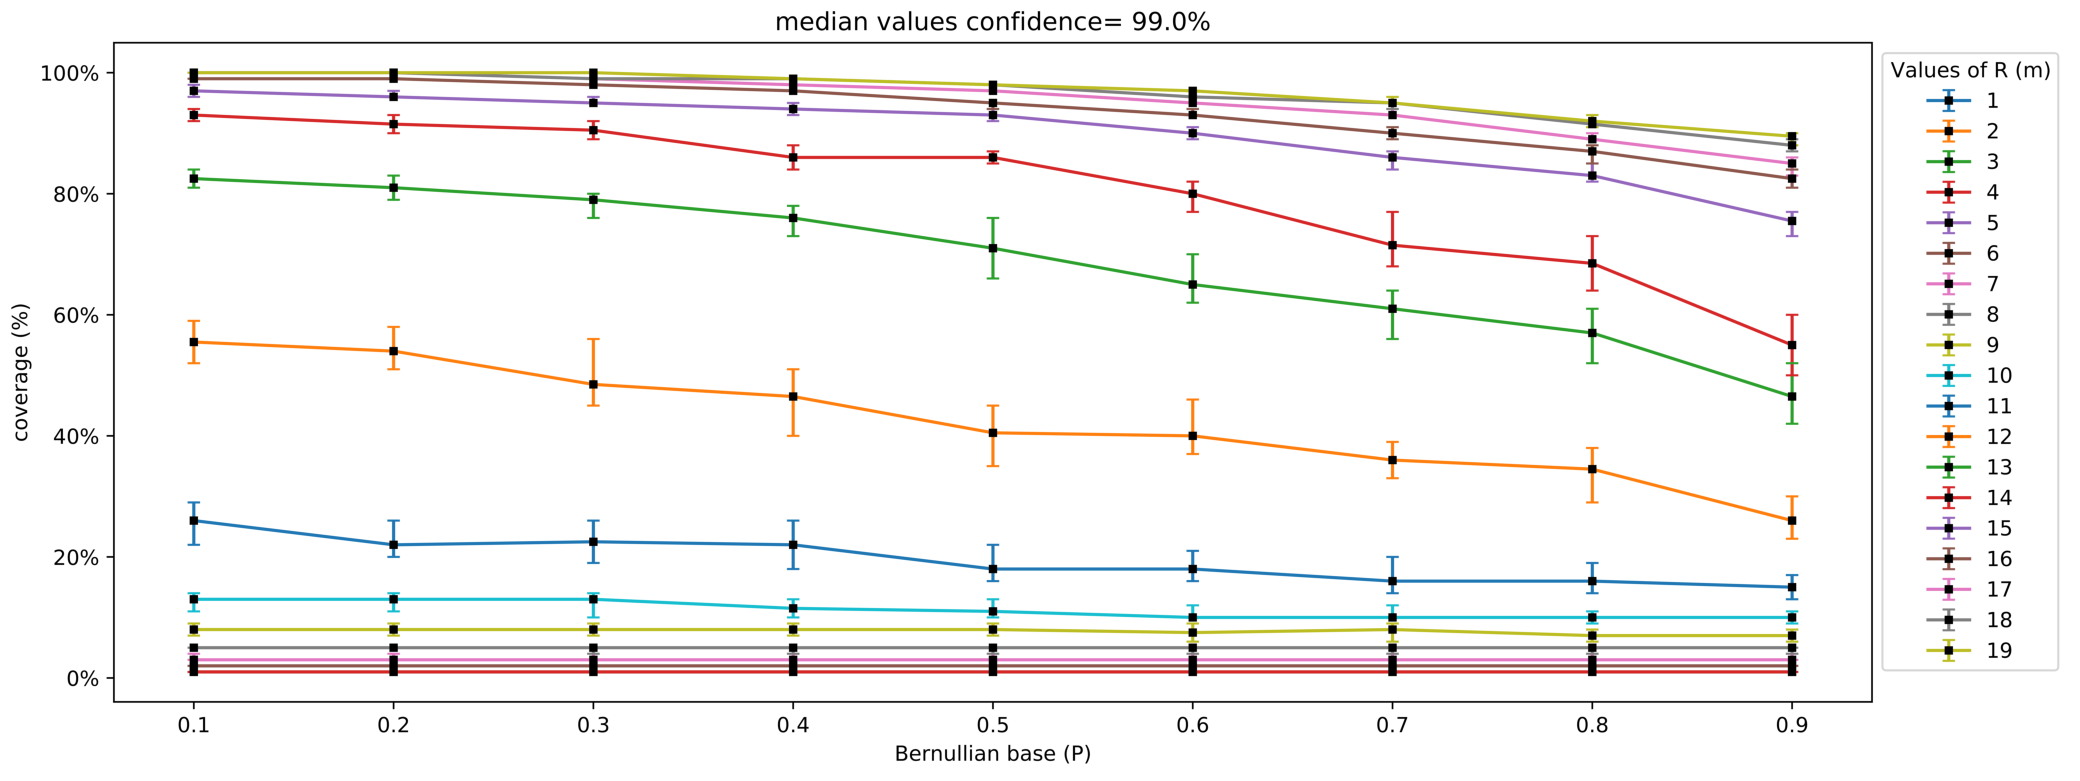
\includegraphics[scale=.42]{img/Big_CovP_median.pdf}
    \end{center}
    \vspace*{-0.5cm}
    \caption{Floorplan coverage as a function of $p$ for different values of $R$}
    \label{fig:floorplancoverage1}
\end{figure}
\noindent
For values of $R$ between $11$ and $15$, the number of collisions has a strong
effect on the coverage percentage; this effect tends to decrease for larger
values of $R$; we know as a matter of fact that for $R \to L\sqrt{2}$ the
coverage tends to $100$\%, independently of any other parameter.\\
\\
Figure \ref{fig:floorplancoverage2} shows the floorplan coverage achieved as a
function of the transmission radius $R$, for different values of the success probability $p$. As expected, accordingly with the previous plot, the
final coverage of the flooplan is deeply influenced by the transmission range $R$.
\begin{figure}[H]
    \begin{center}
        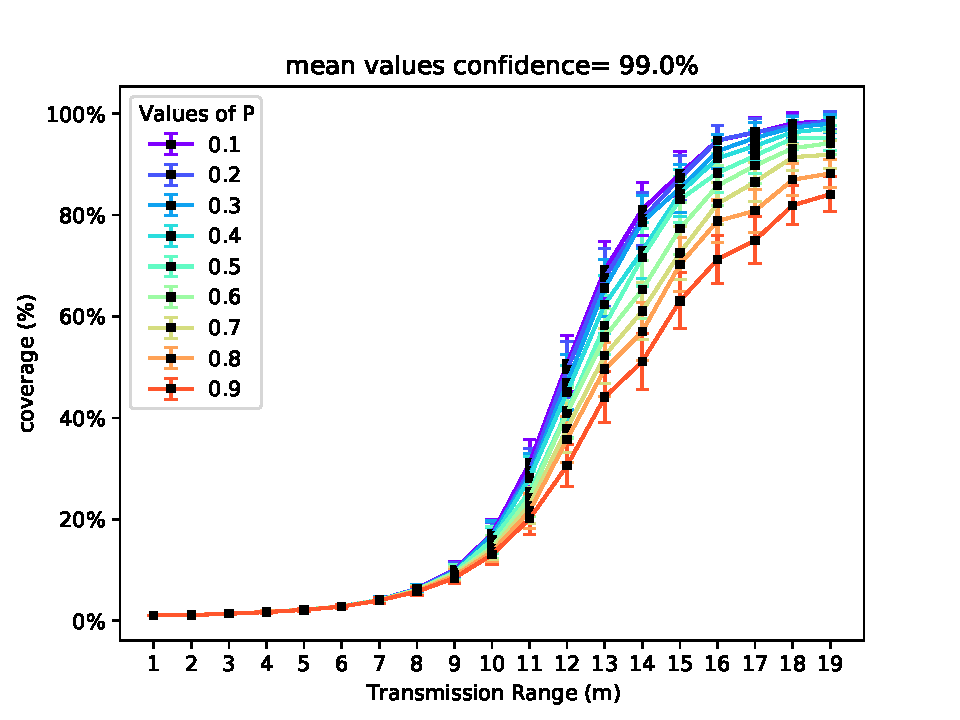
\includegraphics[scale=.75]{img/Big_CovRange_mean.pdf}
    \end{center}
    \vspace*{-0.5cm}
    \caption{Floorplan coverage as a function of $R$ for different values of $p$}
    \label{fig:floorplancoverage2}
\end{figure}
\noindent
%TODO it's better to rephrase and remove 'exponentially' as coverage slows down immediately after r=12 and we ourselves say that it is in fact a sigmoid, not an exponential
In this second plot we can observe that the coverage increases exponentially
with the transmission range. When the transmission range becomes large
($> 16$m), the coverage tends to $100$\%. We recognized the shape of the
sigmoid\footnote{https://mathworld.wolfram.com/SigmoidFunction.html} function,
which can be express as an hyperbolic tangent ($\tanh$); this function is always
increasing and can be manipulated to remain between $0$ and $1$ (like the
parameter we want to fit). A good fit for this curve is given by:
\begin{equation*}
    C = \frac{1+\tanh(aR+b)}{2}
\end{equation*}
where $C$ is the floorplan coverage, $R$ the transmission radius, and $a$ and
$b$ depend on $p$ as shown in the following table:
\begin{center}
\begin{tabular}{ | m{1cm} | m{4cm}| m{4cm} | }
\hline
$p$&$a$&$b$\\
\hline
$0.1$&$0.3628314535334378$&$4.356732935967713$\\
\hline
$0.2$&$0.3572920723369711$&$4.3206795324164835$\\
\hline
$0.3$&$0.34371134773480694$&$4.193385575628803$\\
\hline
$0.4$&$0.3217942874156316$&$3.9814759531755515$\\
\hline
$0.5$&$0.3091448275788839$&$3.88645016495332$\\
\hline
$0.6$&$0.2809863550485405$&$3.6000814495973996$\\
\hline
$0.7$&$0.25932462296148107$&$3.3996924196436975$\\
\hline
$0.8$&$0.23603288616377227$&$3.1648817545125527$\\
\hline
$0.9$&$0.20917405109220505$&$2.929033169711656$\\
\hline
\end{tabular}
\end{center}
\subsection{Duration}
This following figure shows the plot of the duration of the simulation (in
seconds) as a function of $p$, for different values of $R$.
\begin{figure}[H]
    \begin{center}
        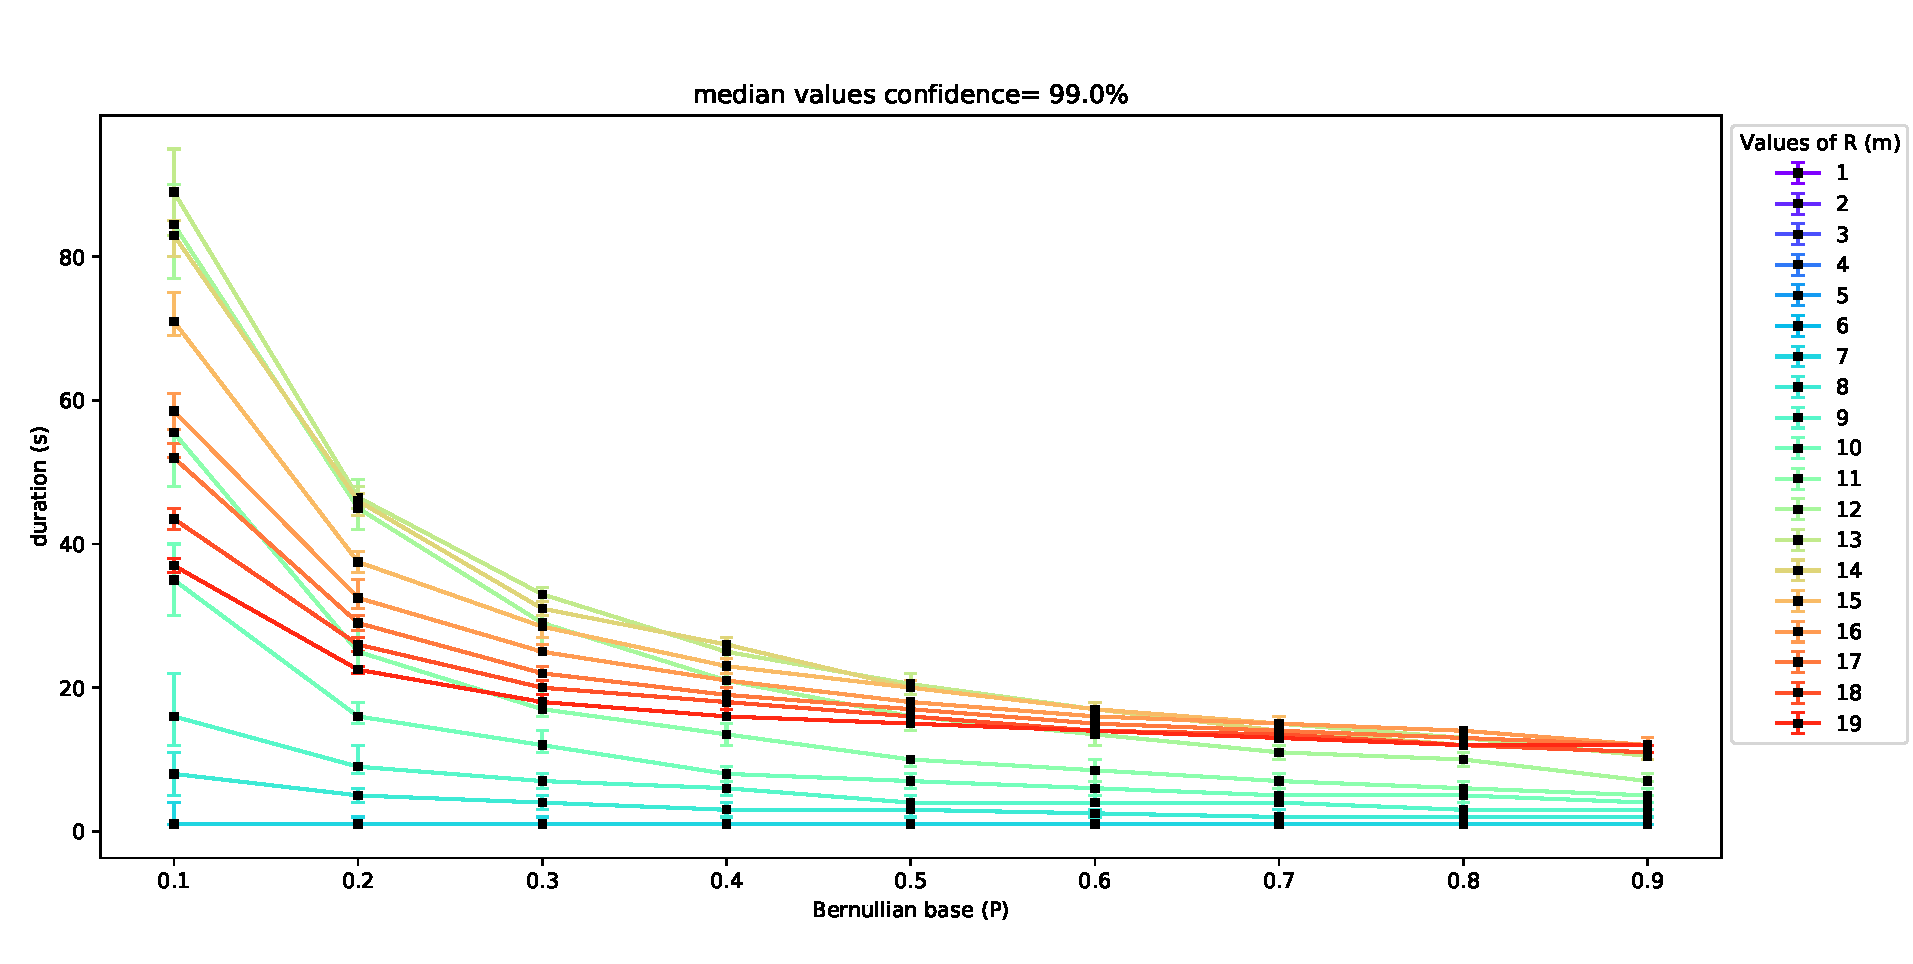
\includegraphics[scale=.51]{img/Big_DurP_median.pdf}
    \end{center}
    \vspace*{-0.5cm}
    \caption{Simulation duration as a function of $p$ for different values of $R$}
    \label{fig:floorplancoverage3}
\end{figure}
\noindent
The simulation duration increases for lower values of $p$; this behaviour can be
explained as a consequence of two main factors:
\begin{itemize}
    \item the probability of retransmission is low, so nodes will spend most
    time slots waiting, without actually transmitting;
    \item with a smaller number of collisions, a higher number of nodes is
    reached; reaching a higher number of nodes requires a higher number of
    retransmissions.
\end{itemize}
We tried to interpolate the curves shown in Figure \ref{fig:floorplancoverage3}
with an hyperbolic function, because it fits well the parameters we want to
model; first of all, the hyperbole tends to infinity as $p$ tends to $0$, and
this is coherent with the reality, because if the probability of retransmission
becomes low, then the duration keeps increasing. If instead $p$ gets close to
$1$, the duration time tends to its minimum. We fit those shapes using:
\begin{equation*}  
    D = \frac{a}{P}+b 
\end{equation*}
where $D$ is the duration of the simulation, $p$ the probability of
retransmission, and $a$ and $b$ depend on $R$ as specified in the following
table:
%TODO too many digits. Better to reformat as the wall of text is not exactly pretty
\begin{center}
\begin{tabular}{ | m{1cm} | m{5cm}| m{5cm} | }
\hline
$R$&$a$&$b$\\
\hline
$1$&$2.4046845625846913$ e-09&$0.999999999244136$\\
\hline
$2$&$2.4046845625846913$ e-09&$0.999999999244136$\\
\hline
$3$&$0.7313966348173997$&$0.9495446821974095$\\
\hline
$4$&$1.3471717522270503$&$0.9454326532617134$\\
\hline
$5$&$1.7744177255115228$&$1.08724762049118$\\
\hline
$6$&$4.652279267805434$&$1.0487610714204172$\\
\hline
$7$&$9.586489452244717$&$1.088347295851843$\\
\hline
$8$&$15.841670397411658$&$1.0643797063994824$\\
\hline
$9$&$28.264640360031194$&$0.49558107430696624$\\
\hline
$10$&$43.141734847778814$&$0.22815570364285975$\\
\hline
$11$&$64.55944043148898$&$-0.07517936077209139$\\
\hline
$12$&$86.56257725232254$&$-0.09919809415424388$\\
\hline
$13$&$89.72686483087844$&$1.2578386401845827$\\
\hline
$14$&$82.15919574473708$&$3.0965825999956778$\\
\hline
$15$&$67.95268283187643$&$5.415446394742158$\\
\hline
$16$&$56.442159145137495$&$6.991880399220213$\\
\hline
$17$&$45.71412729773696$&$7.548465010848107$\\
\hline
$18$&$39.164500694866284$&$7.991652317096266$\\
\hline
$19$&$29.71836400235831$&$9.075854630828385$\\
\hline
\end{tabular}
\end{center}
To be able to compute the correct values the first two entries for $a$ and $b$,
a larger dataset is needed; as a matter of fact, if the transmission range is
too short nodes can not communicate: they are not in reach by each others.\\
\\
The following plot shows the duration of the simulation (in seconds) as a
function of $R$, for different values of $p$.
\begin{figure}[H]
    \begin{center}
        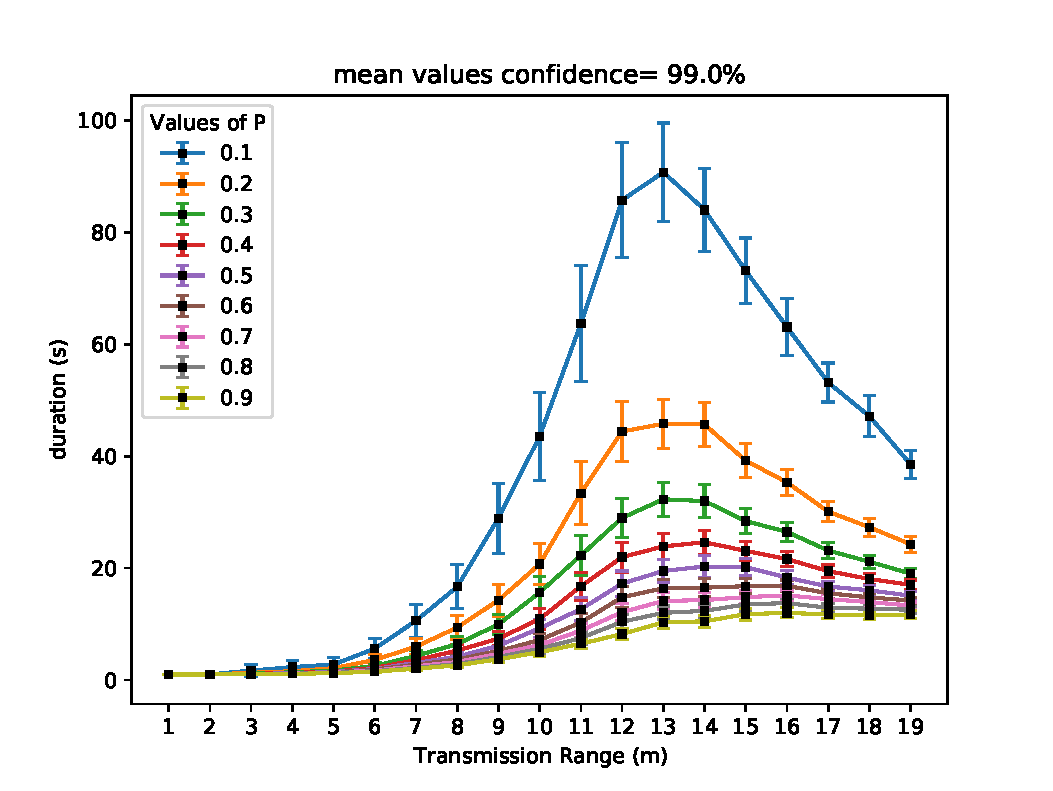
\includegraphics[scale=.7]{img/Big_DurRange_mean.pdf}
    \end{center}
    \vspace*{-0.5cm}
    \caption{Simulation duration as a function of $R$ for different values of $p$}
    \label{fig:floorplancoverage4}
\end{figure}
\noindent
The duration of the simulation tends to increase with the transmission range
reaching a peak around $13$m; the maximum value depends on the probability of
retransmission ($p$);
This is an interesting result, and can be explained by:?%todo
\subsection{Collisions}
This plot show the Number of collisions in function of P, for different values of R.
\begin{figure}[H]
    \begin{center}
        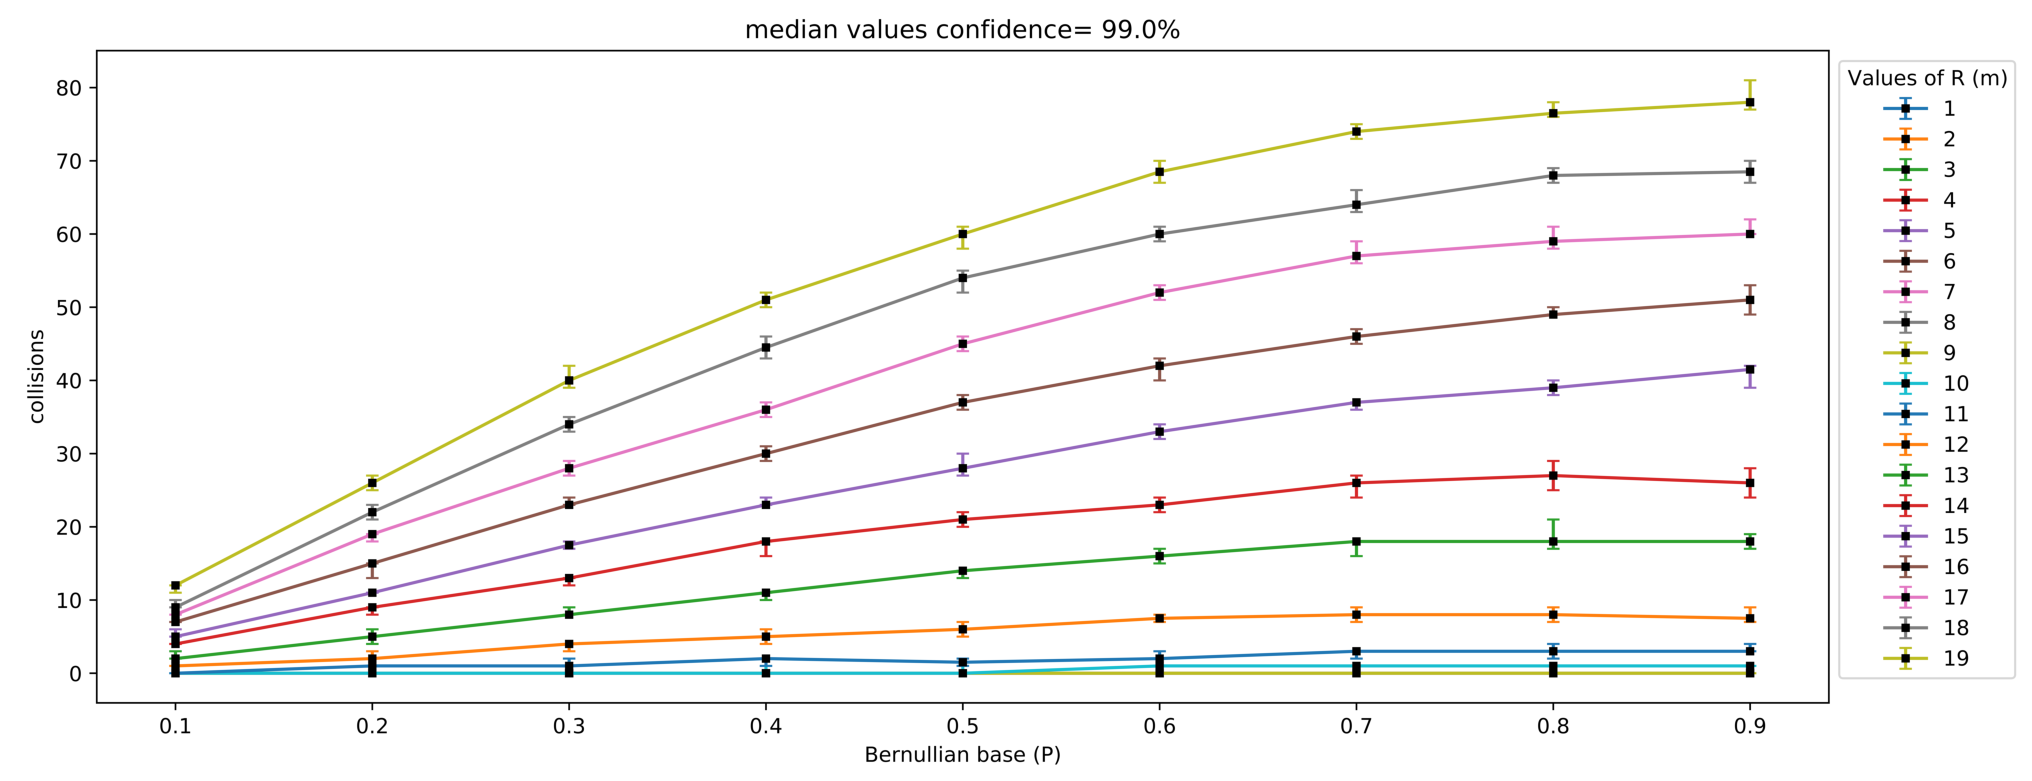
\includegraphics[scale=.4]{img/Big_CollP_median.pdf}
    \end{center}
    \vspace*{-0.5cm}
    \caption{Caption this}
    \label{fig:floorplancoverage5}
\end{figure}
\begin{figure}[H]
    \begin{center}
        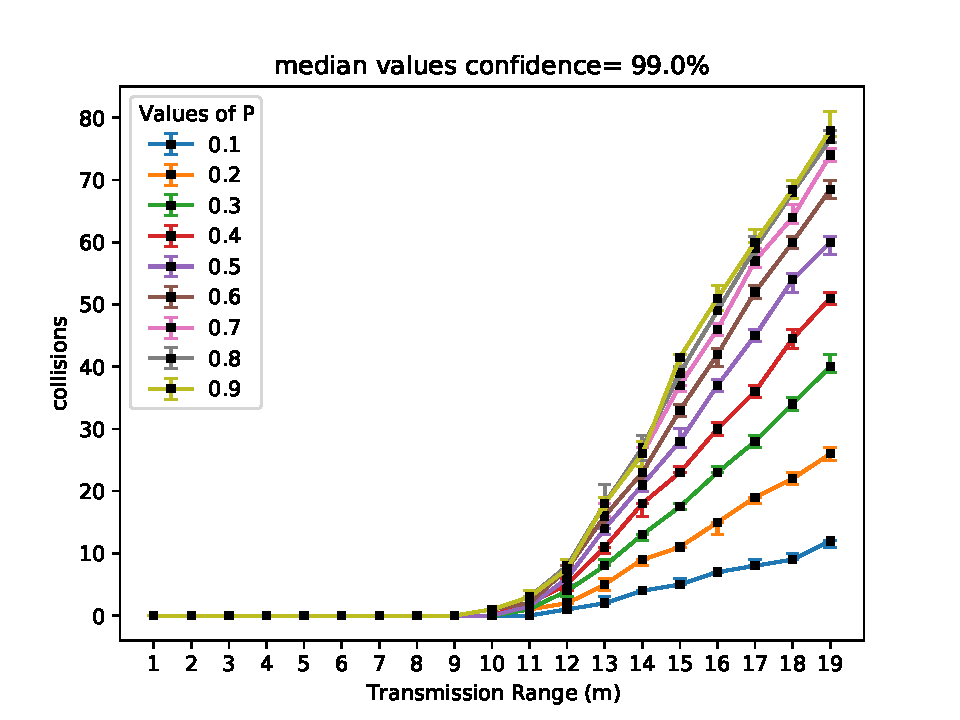
\includegraphics[scale=.7]{img/Big_CollRange_median.pdf}
    \end{center}
    \vspace*{-0.5cm}
    \caption{Caption this}
    \label{fig:floorplancoverage6}
\end{figure}
